\chapter{Modelando decisiones con mayor precisión} \label{cap_5}
En el siguiente capítulo, se explorará una faceta fundamental en la teoría económica y de toma de decisiones, la introducción de un nuevo factor de descuento de la utilidad. Este factor resulta esencial para reflejar de manera más precisa y fiel el comportamiento de los individuos. La premisa fundamental aquí es mejorar la valoración que cada uno de los “yoes” asigna a las distintas opciones y escenarios a lo largo del tiempo, de modo que esta valoración sea un reflejo más ajustado a la realidad y a las complejas dinámicas que influyen en las decisiones.

A lo largo de este capítulo, se examinará en detalle cómo este nuevo factor de descuento de la utilidad contribuye a una toma de decisiones más informada y precisa. Explorándose su impacto en la economía y en la psicología de las decisiones, considerando cómo los seres humanos ponderan las recompensas y consecuencias a lo largo del tiempo. 

En última instancia, este enfoque más preciso y realista en la valoración de la utilidad representa un avance significativo en el entendimiento del comportamiento humano en el contexto de la toma de decisiones económicas. A través de este capítulo, se espera proporcionar una visión más completa, detallada y precisa de cómo las personas evalúan las opciones y cómo esta evaluación puede influir en una amplia gama de decisiones que se toman en la vida cotidiana.


\section{Valor de la recompensa y reforzamiento}
En esta sección se abordará el concepto de valor de la recompensa, los diferentes enfoques para estudiarlo y cómo afecta el reforzamiento en las decisiones.

En principio el factor de descuento se utiliza para “penalizar”  un valor o utilidad que no se encuentra en el momento presente, sino en uno ulterior o futuro. En otras palabras, representa el descuento temporal de una recompensa atrasada.


En \parencite{buritica2016valor} se distinguen dos enfoques para estudiar el valor de la recompensa. Por un lado, un enfoque empírico que reconoce el valor de una recompensa está dado por lo bien que un evento aumenta la posibilidad de que alguien dé una respuesta específica, tal como ratifica  \parencite{mazur2001hyperbolic}. Es como evaluar qué tan efectivo es ese evento para motivar una acción. Por otro lado, un enfoque de inferencia en el cual la noción de valor de la recompensa hace alusión la utilidad como la define \parencite{mankiw2012} que es una medida abstracta de  felicidad o bienestar que se recibe de ciertos bienes.

Para medir el valor de tal recompensa según el enfoque empírico diferentes autores se aprovechan del estudio del  reforzamiento. El reforzamiento, según la definición de \parencite{miltenberger2012behavior}, es el proceso por el cual una conducta se refuerza o fortalece debido a las consecuencias que ocurren después de esa conducta. En \parencite{miltenberger2012behavior} se distinguen dos tipos de reforzamiento, el reforzamiento positivo y el reforzamiento negativo. En el reforzamiento positivo, después de que ocurre una conducta, esta es seguida por la presentación de un estímulo reforzante o un aumento en su intensidad, lo que lleva al fortalecimiento de la conducta. En cambio, en el reforzamiento negativo, después de la ocurrencia de la conducta, esta es seguida por la eliminación de un estímulo aversivo o la reducción de su intensidad, lo que también conduce al fortalecimiento de la conducta. 

El tiempo que transcurre entre que ocurre un comportamiento y la aparición de la consecuencia reforzante será de vital importancia al momento de medir el valor de la recompensa pues cuanto más tiempo transcurra disminuirá la efectividad de una consecuencia como reforzador. 

Otro factor crucial a tener en cuenta, como lo indica \textcite{miltenberger2012behavior}, es el programa de reforzamiento de una conducta. Este programa especifica en qué circunstancias cada respuesta es seguida por un reforzador. Se pueden identificar cuatro tipos distintos de programas de reforzamiento.
\begin{itemize}
    \item \textit{\textbf{Razón fija:}} En este programa, el reforzador se otorga después de un número específico de respuestas. 
    \item \textit{\textbf{Razón variable:}} En este caso, el reforzador se entrega después de un promedio de un número variable de respuestas. 
    \item \textit{\textbf{Intervalo fijo:}} Bajo este programa, el reforzador se otorga por la primera respuesta que ocurre después de un intervalo de tiempo fijo. 
    \item \textit{\textbf{Intervalo variable:}} En este programa, el reforzador se entrega por la primera respuesta después de un intervalo de tiempo variable. 
\end{itemize}

\section{Medición del valor de la recompensa}
En el estudio de \parencite{buritica2016valor}, se realiza un seguimiento de varias mediciones del valor de la recompensa utilizando un enfoque empírico. A continuación, se procederá a examinar algunas de las mediciones que son presentadas en la investigación.

En \parencite{hursh2008economic} se midió el valor de la recompensa en términos de fuerza de la respuesta estableciendo una relación directa entre la fuerza de la respuesta y el valor. Es decir, cuanto mayor es la fuerza de la respuesta, se considera que el valor de la recompensa asociada también es mayor.

En \parencite{verhave1963toward} se utilizó un “valor de equilibrio” para medir el esfuerzo necesario para obtener una recompensa y también para expresar las preferencias relativas de las palomas entre dos programas de refuerzo de razón fija. Las palomas participaron en un experimento con dos componentes de razón fija, uno con razón fija 100 y otro con razón fija 10. El cambio entre estos componentes ocurría cuando las palomas tocaban una tecla de cambio y el valor de equilibrio representaba el punto en el que se estabilizaba su elección.

En \parencite{hodos1961progressive} se propuso medir la fuerza de la recompensa utilizando un programa de razón progresiva donde, cada vez que el sujeto obtiene una recompensa, el número de respuestas necesarias para obtener la siguiente aumenta según un criterio fijo. Descubrió que el punto de quiebre, es decir, el número de respuestas en el cual el sujeto abandona la tarea, dependía de la densidad de la recompensa.

En \parencite{hursh2008economic} se propone una alternativa para medir el valor de la recompensa utilizando un modelo que refleja cómo el consumo de la recompensa responde a los cambios en los costos y beneficios, o lo que se conoce como la “elasticidad de la demanda”. En su modelo cuentan con un parámetro que representa la elasticidad para toda la curva. Tal parámetro, se considera como un reflejo del valor de la recompensa. 

Luego en \parencite{buritica2016valor} se distingue el valor de la recompensa como constructo hipotético siendo que el valor de 
la recompensa existe, en alguna medida, más allá de lo observado y como variable interviniente siendo parte de un conjunto de relaciones entre variables. En el caso del constructo hipotético cabe destacar el estudio de \parencite{chib2009evidence},  que sostiene que en el cerebro, los bienes son procesados en áreas similares, tal como si hubiera una especie de “moneda” común que representara el valor y que pudiera ser utilizada para comparar distintos bienes y tomar decisiones.

\section{Recompensas diferidas y descuento}
Tal como se ha señalado previamente en \parencite{miltenberger2012behavior}, al medir el valor de la recompensa, es importante tener en cuenta que a medida que aumenta el tiempo entre un comportamiento y la consecuencia reforzante, la efectividad de esta consecuencia como refuerzo disminuirá.

En \parencite{buritica2016valor} se resaltan dos lineas de estudio que se derivan del retraso en la obtención de la recompensa. La primera línea, busca explicar que la disminución en la efectividad de una recompensa retrasada se debe a una reducción en la tasa global de reforzamiento. La segunda línea, sugiere que hay un fenómeno de descuento temporal en el cual el valor de la recompensa disminuye a medida que se retrasa su entrega.

Siguiendo la linea del descuento temporal, en \parencite{madden2010delaydiscounting} se hace un estudio exhaustivo sobre la evolución de las funciones que reflejan el descuento. Se describe el descuento temporal como parte de un proceso de decisiones impulsivas en el cual el valor subjetivo de una cantidad pequeña ahora es mayor que el de una cantidad mayor luego. 

Una de las fórmulas propuesta para describir tal descuento es la de descuento exponencial propuesta en \parencite{Samuelson37} la cual fue ampliamente utilizada. 
Además, debe destacarse, como se menciona en \parencite{myerson1995discounting}, que en dicho modelo se postula que el valor de una recompensa futura es descontado en función del riesgo asociado con su espera, implicando, por consiguiente, la existencia de una tasa de riesgo constante relacionada con el potencial fracaso en su obtención. Este modelo se expresa mediante la siguiente ecuación:
%
\begin{equation}
\label{Samuelson_eq}
    V=A \exp(-\rho t),
\end{equation}
%
donde $V$ es el valor presente de una recompensa futura, $A$ el monto de tal recompensa, $t$ es el delay o retraso a su obtención y  $\rho$ es un parámetro que indica la tasa de riesgo constante. Es relevante destacar que en el contexto del modelo de consumo intertemporal estudiado, $\exp(-\rho t)$ es empleado como la base para medir posteriormente la desviación en los factores de ponderación futuros.

En \parencite{madden2010delaydiscounting} se señala que se han registrado desvíos sistemáticos de la función \ref{Samuelson_eq} de descuento exponencial en investigaciones con sujetos humanos \parencite{myerson1995discounting,kirby1997bidding} y con animales \parencite{mazur1997choice}. 
Por tanto, \parencite{ainslie1975specious,mazur1987adjusting} proponen la siguiente función de descuento hiperbólica, que se ajusta de manera más precisa al comportamiento tanto de las personas como de los animales
%
\begin{equation}
\label{hiperbolic_eq}
    V=\dfrac{A}{1+\eta t},
\end{equation}
%
donde $V$ el valor presente de un recompensa futura, $A$ el monto de tal recompensa, $t$ es el delay o retraso a su obtención y  $\eta$ es un parámetro que que rige la tasa de disminución del valor, el cual es análogo al parámetro $\rho$ de (\ref{Samuelson_eq}). Como se explica en \parencite{myerson1995discounting} si se ajusta a los mismos datos, la hipérbola decrecerá inicialmente (en intervalos cortos) más rápido que la función exponencial, pero luego (en intervalos largos) decrecerá más lentamente. En el contexto del modelo de consumo intertemporal estudiado, la función de descuento principal utilizada es ${1}/{(1+\eta t)}$.

En el estudio de \parencite{myerson1995discounting} se destaca que la función hiperbólica de descuento es más efectiva que la exponencial al ajustar datos de grupo, como se señala en el trabajo previo de \parencite{rachlin1991subjective}. Sin embargo, en \parencite{myerson1995discounting} se advierte también que la forma de la función que mejor describe los datos agregados no siempre coincide con la forma que describe los datos no agregados, como se observa en estudios anteriores \parencite{estes1956problem,sidman1952note}. Por lo tanto, no se ha demostrado que el modelo hiperbólico proporcione una descripción más precisa de los datos cuando se trata de sujetos individuales que un modelo exponencial. 

Como no está demostrado, en \parencite{myerson1995discounting} se reanalizan los datos de investigaciones previas realizadas por ellos en \parencite{green1994discounting} para comparar el comportamiento de individuos y su ajuste en funciones de descuentos hiperbólicas y exponenciales. Los participantes en el estudio original eran 12 estudiantes universitarios. El experimento se llevó a cabo de forma individual en una habitación tranquila. Cada participante tenía ante ellos dos juegos de cartas. Uno de los juegos se ubicaba a la derecha y representaba una cantidad fija de dinero (\$1000 o \$10,000), pero esta cantidad estaría sujeta a un retraso previamente establecido antes de recibirla. El otro juego estaba situado a la izquierda y ofrecía una cantidad que variaba entre el 0.1\% y el 100\% de la cantidad fija, pero esta cantidad estaba disponible de inmediato. A los participantes se les presentaba simultáneamente una carta de cada uno de los mazos, y se les pedía que eligieran entre la cantidad fija con retraso y la cantidad variable de entrega inmediata. Para cada cantidad fija y cada período de retraso, calcularon el promedio de la cantidad inmediata en la que el participante cambió su preferencia de la recompensa inmediata a la retrasada en la valoración descendente, así como la cantidad en la que el participante cambió su preferencia de la recompensa retrasada a la inmediata en la valoración ascendente. 

Como resultado, encontraron que el descuento hiperbólico se ajusta mejor a los datos que el descuento exponencial. Además, al revisar tanto los datos agregados como los de algunos sujetos individuales, observaron que el valor presente de una recompensa retrasada disminuye menos abruptamente en retrasos largos de lo que se predice mediante las funciones de descuento exponencial o hiperbólico. Debido a ello, propusieron un modelo cuasi-hiperbólico de dos parámetros que también puede captar la forma de la disminución del valor actual y que fue presentado previamente en 
%
\parencite{green1994discounting,loewenstein1992anomalies}:
\begin{equation}
\label{cuasi_hiper_eq}
    V= \frac{A}{(1+ \eta t)^j},
\end{equation}
%
donde $V$ el valor presente de un recompensa futura, $A$ el monto de tal recompensa, $t$ es el delay o retraso a su obtención y  $\eta$ es un parámetro que que rige la tasa de disminución del valor, el cual es análogo al parámetro $\eta$ de (\ref{hiperbolic_eq}) y al parámetro $\rho$ de (\ref{Samuelson_eq}). El parámetro $j$ modifica la forma de la hipérbola de tal manera que cuando $j$ es menor que 1.0, la curva se aplana, nivelándose a medida que $t$ (el retraso) aumenta.  

En \parencite{myerson1995discounting} se demuestra que el descuento cuasi hiperbólico (\ref{cuasi_hiper_eq}) no solo se ajusta significativamente mejor a los datos, sino que también, describe el descuento temporal de cada individuo de manera más precisa que el modelo exponencial. En adición, este modelo permite reflejar gracias al parámetro del exponente que el valor presente disminuye menos abruptamente en retrasos largos. Adicionalmente, llevaron a cabo una búsqueda para determinar el valor del parámetro $j$ que mejor reflejaba el comportamiento de los individuos, y descubrieron que en 8 de los 12 sujetos, $j$ era significativamente diferente de 1.0. De estos 8 sujetos, en 7 de ellos, $j$ resultó ser significativamente inferior a 1.0. En base a los resultados, se puede concluir que el parámetro $j$ se encuentra en el intervalo $(0,1]$, ya que si fuera menor que 0, perdería su función de descontar y no es mayor a 1 de acuerdo con los hallazgos empíricos. 

En las siguientes secciones, se analizará la función (\ref{cuasi_hiper_eq}) propuesta por \textcite{myerson1995discounting} en el marco del modelo de consumo intertemporal. Primero, se corroborará si garantiza una ponderación futura fuerte. Luego, se verificará si cumple con el sesgo de presente, lo que asegurará que se cumplan las reversiones de preferencias. Después, se evaluará si respeta la condición de Pareto. Por último, se comprobará si respeta la concavidad del plan de consumo. Si se cumplen las condiciones, se podrá afirmar que la función cuasi-hiperbólica es adecuada para el modelo y que proporciona mejores resultados según la evidencia empírica.

\section{Revisión de la ponderación futura fuerte}
En esta sección, se procederá a examinar la función de descuento (\ref{cuasi_hiper_eq}) con el fin de determinar la dinámica de los parámetros $\eta$ y $j$ que garantice una ponderación futura fuerte.

La función de descuento cuasi-hiperbólica, tal como fue propuesta en \parencite{myerson1995discounting}, se expresa de la siguiente manera:
\begin{equation}
    \label{c_hiper}
    D(t)=\dfrac{1}{(1+\eta t)^j}.
\end{equation}

El resultado de que los valores del parámetro $j$ se encuentren en el rango de 0 a 1 se conservará, ya que esto se deriva de los hallazgos del estudio empírico.

Como primer paso, se busca identificar los valores de $\eta>0$ y $\rho>0$ con $j \in (0,1)$ para los cuales la funcional de descuento exponencial es inferior a la cuasi-hiperbólica, con el fin de posteriormente determinar el valor óptimo de $\rho$. 

Es importante destacar que cuando $j$ es igual a 1, la ecuación (\ref{c_hiper}) es idéntica a (\ref{hiperbolic_eq}) y en aras de mantener la coherencia del modelo, se asume que el parámetro óptimo $\rho$ es igual a $\eta$ y posteriormente se verificará la validez de esta afirmación.

Siendo $\rho^{\ast}=\eta$ entonces debido a la expresión (\ref{eq 4}) se busca que
\begin{equation}
\label{cap 5 condi exp}
    D(t) \geq \exp(-\eta t) \Rightarrow
\dfrac{1}{(1+\eta t)^j} \geq \exp(-\eta t)
\end{equation}
%
lo cual es equivalente a
$$\exp(\eta t) \geq (1+ \eta t)^j.$$
%
En $t=0$ vale la igualdad y por tanto bastará con que la derivada que es la tasa de cambio de $\exp(\eta t)$ sea mayor o igual que la derivada de  $(1+ \eta t)^j$
$$\dfrac{d}{dt}\exp(\eta t) \geq \dfrac{d}{dt} (1+ \eta t)^j \Rightarrow
\eta \exp(\eta t) \geq j (1+ \eta t)^{j-1} \eta $$
%
se simplifica y se obtiene
$$\exp(\eta t) \geq j (1+ \eta t)^{j-1}.$$
%
Analizando $j (1+ \eta t)^{j-1}$ si se tiene en consideración que $j \in (0,1)$
$$j (1+ \eta t)^{j-1}= j \overbrace{\dfrac{1}{(1+ \eta t)^{1-j}}}^{\in (0,1]} < 1.$$
%
Puesto que queda evidenciado que $1 > j (1+ \eta t)^{j-1}$ entonces es prueba suficiente para mostrar que $\exp(\eta t) \geq (1+ \eta t)^j$ debido a que 
$\exp(\eta t) \geq 1$ y por tanto
\begin{equation}
\label{eq sec 5.4}
j (1+ \eta t)^{j-1}<1 \leq \exp(\eta t) .
\end{equation}

Entonces, al cumplirse (\ref{eq sec 5.4}) se verifica que con $\rho = \eta$, la función de descuento supera a la función exponencial. Sin embargo, es de interés  determinar si existe algún valor aún menor que $\eta$ que mantenga la función de descuento por encima de la función exponencial. Se supondrá que $\rho$ está en el intervalo $(0, \eta)$ y
%
$$\dfrac{1}{(1+\eta t)^j} \geq \exp(-\rho t)$$
siendo $t\geq 0$. En consecuencia, el inverso multiplicativo de la función exponencial supera al de la función de descuento de tal manera que 
$$ \exp(\rho t)\geq (1+\eta t)^j.$$
%
De manera similar a lo demostrado en \ref{ex 2}, se definirá una función $f(t,\rho)$ que evalúa la diferencia entre el inverso multiplicativo de la función exponencial y el de la función de descuento del siguiente modo
%
$$f(t,\rho)=\exp(\rho t)-(1+\eta t)^j.$$
%
Para evaluar si cumple con los requisitos, resultará de interés buscar los extremos de la función y en caso de que el extremo genere un valor negativo, será suficiente como prueba para afirmar que el parámetro óptimo $\rho$ es igual a $\eta$.

Por tanto, se tiene

$$f(0,\rho)=\exp(0)-(1)^j=0, \quad 
\dfrac{d}{dt}f(t,\rho)=\rho\exp(\rho t)-j(1+\eta t)^{j-1}\eta.$$
y además
$$\dfrac{d}{dt} \dfrac{d}{dt}f(t,\rho)=\rho^2 exp(\rho t)-j (j-1)(1+\eta t)^{j-2}\eta^2>0 .$$
%
De este análisis se deducen dos conclusiones: 1) no es factible resolver de manera analítica la primera derivada igualándola a cero pues queda una ecuación trascendente y 2) pueden existir mínimos dependiendo de los valores de $j$, $\eta$ y $\rho$ (por ejemplo $t=0$ es un mínimo si $\rho=j \eta$). 
% Ahora, solo resta determinar si dicho mínimo se sitúa en $t \geq 0$ y si es negativo.

% Con el fin de alcanzar este objetivo, se utilizará el algoritmo de descenso del gradiente, el cual indica que, para una función $f(x)$, se puede aproximar de forma iterativa al valor mínimo empleando un coeficiente de aprendizaje $\alpha$ a través de la siguiente ecuación:
% %
% $$x_{n+1}=x_n - \alpha \nabla f(x_n).$$
% %
% En este escenario, se establecerá el coeficiente de aprendizaje como $\alpha=1$, se tomará un valor inicial de $t_0=0$ y se llevará a cabo una iteración para su evaluación.
% $$t_0=0 \Rightarrow f(0,\rho)=\exp(0)-(1)^j=0.$$
% $$t_1=0 - \dfrac{d}{dt}f(0,\rho)=0 - \left(\rho - j \eta \right)=j \eta - \rho. $$
% $$t_1=j \eta - \rho \Rightarrow f(j \eta - \rho ,\rho)=\rho\exp(\rho (j \eta - \rho))-j(1+\eta (j \eta - \rho))^{j-1}\eta.$$

% Dado que $j \eta - \rho$ puede tomar valores negativos, nulos o positivos, no tiene sentido continuar con las iteraciones, ya que su evaluación dependerá de los valores específicos de $j$, $\eta$ y $\rho$. 

Por lo tanto, podemos concluir que existen valores del parámetro $\rho$ que son menores que $\eta$ y que cumplen (\ref{cap 5 condi exp}) pero no se pueden deducir mediante una fórmula general, ya que no se puede despejar $\rho$ para ellos. En consecuencia, consideramos que $\rho=\eta$ es un subóptimo, pero se continuará trabajando con este valor, ya que garantiza que la función de descuento cuasi-hiperbólica sea siempre mayor que la función exponencial y además, mantiene la coherencia con el caso hiperbólico en el cual $j=1$.

\section{Revisión del sesgo de presente}
\label{section_sesgo_presente}
En esta sección, se analizará si el descuento cuasi-hiperbólico (\ref{c_hiper}) cumple con la condición de sesgo de presente establecida en (\ref{fpmeqbias}).

La condición que debe cumplirse, para que un hogar manifieste sesgo de presente, lo que también implica la reversión de preferencia, es la siguiente
\begin{equation*}
\varepsilon'(0) \leq  \dfrac{\varepsilon'(t)}{1+ \varepsilon(t)},
\end{equation*}
además, debe cumplirse $\varepsilon(t) > -1$.

A partir de la ecuación (\ref{eq 3}), se procede al cálculo de $\varepsilon(t)$ y $\varepsilon'(t)$  para el descuento cuasi-hiperbólico. %
%y considerando el subóptimo $\rho=\eta>0$
 El factor de ponderación futuro $\varepsilon(t)$ resulta
 
\begin{equation}
    \label{var_ep_t}
    \varepsilon(t)=\exp(\rho t)D(t)-1=\dfrac{\exp(\rho t)}{(1+\eta t)^j}-1=\exp(\rho t)(1+\eta t)^{-j}-1.
\end{equation}
%
$\varepsilon'(t)$ se puede expresar como
\begin{equation}
    \label{deriv_var_ep_t}
    \varepsilon'(t)=\dfrac{\rho\exp(\rho t)}{(1+\eta t)^{j}}-\dfrac{j \eta \exp(\rho t) }{(1+\eta t)^{j+1}}.
\end{equation}
se valúa en $t=0$
\begin{equation}
    \label{deriv_var_ep_0}
\varepsilon'(0)=\rho-j \eta.
\end{equation}
Se procede a calcular $\dfrac{\varepsilon'(t)}{1+ \varepsilon(t)}$ resultando en
\begin{equation}
    \label{deriv_var_mu_t}
    \dfrac{\varepsilon'(t)}{1+ \varepsilon(t)}=\left(\dfrac{\rho\exp(\rho t)}{(1+\eta t)^{j}}-\dfrac{j \eta \exp(\rho t) }{(1+\eta t)^{j+1}} \right)\dfrac{(1+\eta t)^j}{\exp(\rho t)}=\rho - \dfrac{j \eta}{(1+\eta t)}.
    \end{equation}
Se evaluará entonces la condición de sesgo de presente considerando que los parámetros $\rho>0$, $\eta>0$ y $j \in (0,1)$ 
$$\rho-j \eta \leq \rho - \dfrac{j \eta}{(1+\eta t)}\Rightarrow \dfrac{j \eta}{(1+\eta t)} \leq j \eta.$$
Dado que $(1+\eta t) \geq 1$, la desigualdad está demostrada. 

Se analiza, por ultimo, la condición 
$\varepsilon(t)>-1$.
Dado que $\varepsilon(t)=\exp(\rho t)(1+\eta t)^{-j}-1$, tal como se muestra en (\ref{var_ep_t}),
%
$$\exp(\rho t)(1+\eta t)^{-j}-1>-1,$$
%
lo cual es equivalente a
%
$$\exp(\rho t)(1+\eta t)^{-j}>0.$$
%
Considerando que los parámetros $t\geq 0$, $\rho>0$, $\eta>0$ y $j\in (0,1)$, se puede establecer que $\exp(\rho t)\geq 1$ y $(1+\eta t)^{-j}\geq 1$. Por lo tanto, la siguiente condición $\varepsilon(t)>-1$ se encuentra satisfecha. 

En conclusión, se confirma que el descuento cuasi-hiperbólico cumple con el sesgo de presente.

\section{Revisión de la condición de Pareto}
En esta sección, se llevará a cabo un análisis para determinar si el descuento cuasi-hiperbólico (\ref{c_hiper}) cumple con la condición de óptimo de Pareto, tal como se establece en (\ref{eq 67}), con el propósito de que prevalezca el plan inicial por encima de los demás planes.

La condición de óptimo de Pareto, como se ha explicado previamente en \parencite{feigenbaum2021deviation}, es necesaria pero no suficiente y se expresa de la siguiente manera
\begin{equation}
\label{basic_condi_pareto}
D(T)> \exp \left( - \ds \int_0^T \dfrac{(1- D(t)) dt}{\ds \int_0^{t} D(s) ds}\right).    
\end{equation}

Es equivalente a que el consumo terminal siguiendo el plan inicial sea mayor o igual al consumo terminal realizado.
Para verificar su cumplimiento se analizará cada componente por separado. 
%
El primero de ellos $D(T)$ indica el descuento de un valor o utilidad en la edad terminal $T$ y se expresa de la siguiente manera 
$$D(T)=\dfrac{1}{(1+\eta T)^j}.$$
%
El segundo de ellos, es una función de la propensión marginal a consumir, tal cual se ve en (\ref{eq 47}),(\ref{eq 51}) y (\ref{eq 65}). Para hallar una equivalencia para la integral, se analizarán minuciosamente todas sus composiciones.

El desarrollo de cada integral que se presentará en esta sección se halla en el Apéndice \ref{Apendice_G}. La integral del denominador equivale a
$$\ds \int_0^{t} D(s) ds=\ds \int_0^{t} \dfrac{1}{(1+\eta s)^j} ds=\dfrac{1}{\eta(1-j)}((1+\eta t)^{1-j}-1).$$

La integral dentro de la exponencial de (\ref{basic_condi_pareto}) equivale a
\begin{equation}
\label{right_int_condi_pareto}\ds \int_0^T \dfrac{(1- D(t)) dt}{\ds \int_0^{t} D(s) ds} =
\ds \int_0^{t} \dfrac{1 - \dfrac{1}{(1+\eta t)^j}}{\dfrac{1}{\eta(1-j)}((1+\eta t)^{1-j}-1)} dt,\end{equation}
que se puede expresar equivalentemente del siguiente modo
\begin{equation*}
        \ds \int_0^{T} \dfrac{1 - \dfrac{1}{(1+\eta t)^j}}{\dfrac{1}{\eta(1-j)}((1+\eta t)^{1-j}-1)} dt=
\end{equation*}
\begin{equation*}
        =\ds \int_0^{T} \dfrac{1}{\dfrac{1}{\eta(1-j)}((1+\eta t)^{1-j}-1)} dt-\ln\left( (1+\eta T)^{1-j}-1\right)+\lim_{t \to 0} \ln\left( (1+\eta t)^{1-j}-1\right)
\end{equation*}

Cabe destacar que para la primera integral no se pudo obtener una expresión general por lo cual se buscará una expresión alternativa que permita resolver la inecuación. Para ello se le asignará el nombre $I(t)$ al integrando de (\ref{right_int_condi_pareto}) y la inecuación se puede escribir del siguiente modo 
$$\dfrac{1}{(1+\eta T)^j}> \exp\left(-\ds \int_0^{T}I(t)dt
\right),$$
se usan propiedades de la potencia y se obtiene
$$\dfrac{1}{(1+\eta T)^j}>\dfrac{1}{\exp\left(\ds \int_0^{T}I(t)dt\right)}. $$
Dado que no se ha encontrado una expresión general para la integral de $I(t)$, se buscará una función $q(t)$ que sea comparable tanto con $I(t)$ como con $D(T)$, de manera que sea posible corroborar la inecuación original (\ref{basic_condi_pareto}).

Notar que $q(t)>0$ si se considera que en el integrando de (\ref{right_int_condi_pareto}) se verifica que el numerador es positivo ya que $\dfrac{1}{(1+\eta t)^j}<0$ y que el denominador es positivo dado que $\eta(1-j)>0$ y $(1+\eta t)^{1-j}>1$.

Si se verifica que $I(t)>0$ y se cumple
$$ \dfrac{1}{\exp\left(\ds \int_0^{T}q(t)dt\right)} >   \dfrac{1}{\exp\left(\ds \int_0^{T}I(t)dt\right)},$$
o equivalentemente
\begin{equation}
    \label{sub_condi_pare_cuasi}
\ds \int_0^{T}q(t)dt <  \ds \int_0^{T}I(t)dt, 
\end{equation}
%
si se logra demostrar también que 
\begin{equation}
\label{sub_condi_pare_cuasi2}
    \dfrac{1}{(1+\eta T)^j} >   \dfrac{1}{\exp\left(\ds \int_0^{T}q(t)dt\right)}, 
\end{equation}
%
entonces se corrobora (\ref{basic_condi_pareto}) que es equivalente a
\begin{equation}
\label{basic_condi_pareto_2}
    \dfrac{1}{(1+\eta T)^j} >  \dfrac{1}{\exp\left(\ds \int_0^{T}I(t)dt\right)}.
\end{equation}

\subsection{Primera subcondición}
En esta subsección, se procederá a realizar un análisis detallado de la subcondición (\ref{sub_condi_pare_cuasi}), con el propósito de identificar una función $q(t)>0$ que cumpla con los requisitos establecidos.
Para determinar $q(t)$ se propone que cumpla lo siguiente
\begin{equation*}
    \dfrac{1}{(1+\eta T)^j+1} =  \dfrac{1}{\exp\left(\ds \int_0^{T}q(t)dt\right)}.
\end{equation*}
Pues bien, si se llega a corroborar lo mencionado, entonces es evidente que la función cumplirá con (\ref{basic_condi_pareto}) y (\ref{basic_condi_pareto_2}), dado que $\dfrac{1}{(1+\eta T)^j} > \dfrac{1}{(1+\eta T)^j+1}$.
%
\begin{equation}
\label{q_de_t_expo_integral}
    (1+\eta T)^j+1 =  \exp\left(\ds \int_0^{T}q(t)dt\right).
\end{equation}
se aplican logaritmos a ambos lados
\begin{equation*}
    \ln \left((1+\eta T)^j+1\right) =   \int_0^{T}q(t)dt.
\end{equation*}
se deriva para $t$
\begin{equation*}
    \dfrac{d}{dt} \left(\ln \left((1+\eta T)^j+1\right)\right) =   \dfrac{d}{dt} \left(\int_0^{T}q(t)dt\right).
\end{equation*}
se despeja $q(T)$
\begin{equation}
\label{q_de_T}
    \dfrac{j\eta(1+\eta T)^{j-1}}{(1+\eta T)^j+1} =   q(T).
\end{equation}

Cabe notar que $q(T)>0$ considerando que el numerador es positivo puesto que $\eta>0$, $j\in (0,1)$ y $(1+\eta T)^{j-1} \geq 1$ y que el denominador es positivo dado que $(1+\eta T)^{j-1} \geq 1$

Luego de haber encontrado la función $q(t)$ que cumple con los requisitos se debe comprobar
%
$$\ds \int_0^{T}\dfrac{j\eta(1+\eta t)^{j-1}}{(1+\eta t)^j+1}dt<\ds \int_0^{T} \dfrac{1 - \dfrac{1}{(1+\eta t)^j}}{\dfrac{1}{\eta(1-j)}((1+\eta t)^{1-j}-1)} dt.$$
%
Dado que $\eta>0$ y $j\in (0,1)$, entonces es fácil comprobar $1+\eta t \geq 1$ y $\eta(1-j)>0$ para $t>0$ puesto que en $t=0$ no está definido el dominio de $I(t)$. Para $t>0$ vale que $I(t)> 0$ y $q(t)> 0$. Si ambos son positivos y existe una desigualdad estricta entre ellos para todo $t > 0$, entonces al compararlos directamente se puede demostrar la desigualdad original. Para ello, se aplicará la generalización del Teorema Fundamental del Cálculo.
%
$$\dfrac{d}{dT}\left(\ds \int_0^{T}\dfrac{j\eta(1+\eta t)^{j-1}}{(1+\eta t)^j+1}dt\right)<\dfrac{d}{dT}\left(\ds \ds \int_0^{T} \dfrac{1 - \dfrac{1}{(1+\eta t)^j}}{\dfrac{1}{\eta(1-j)}((1+\eta t)^{1-j}-1)} dt\right).$$
$$\dfrac{j\eta(1+\eta T)^{j-1}}{(1+\eta T)^j+1}<\dfrac{1 - \dfrac{1}{(1+\eta T)^j}}{\dfrac{1}{\eta(1-j)}((1+\eta T)^{1-j}-1)}.$$
%
Se considera $T>0$ se puede renombrar $k=1+ \eta T>1$ y por ello reescribir la desigualdad del siguiente modo
\begin{equation}
\label{eq cap 5 dif}
    \dfrac{j\eta k^{j-1}}{k^j+1}<\dfrac{1 - \dfrac{1}{k^j}}{\dfrac{1}{\eta(1-j)}(k^{1-j}-1)}.
\end{equation}
Se simplifica y se reformula la desigualdad (\ref{eq cap 5 dif})  
$$\dfrac{j k^{j-1}}{k^j+1}<\dfrac{(1-j) \left(1 - \dfrac{1}{k^j}\right)}{k^{1-j}-1}.$$
% $$j k^{j-1} \left(k^{1-j}-1\right)<(1-j) \left(1 - \dfrac{1}{k^j}\right) \left(k^j+1\right).$$
% $$j \left(1-k^{j-1} \right)<(1-j) \left(k^j- k^{-j}\right) .$$
Dada la complejidad de la desigualdad, se la analiza tomando en consideración la diferencia $d(k,j)$ de los términos que la componen (el término a derecha menos el término a izquierda), la cual deberá ser un valor mayor a cero. Este análisis se llevará a cabo gráficamente, considerando valores específicos para $k>0$ (pero sabiendo que $k>1$) y valores de $j \in (0,1)$. 

$$d(k,j) = \dfrac{(1-j) \left(1 - \dfrac{1}{k^j}\right)}{k^{1-j}-1} - \dfrac{j k^{j-1}}{k^j+1}$$
\begin{figure}[!h]
\begin{center}
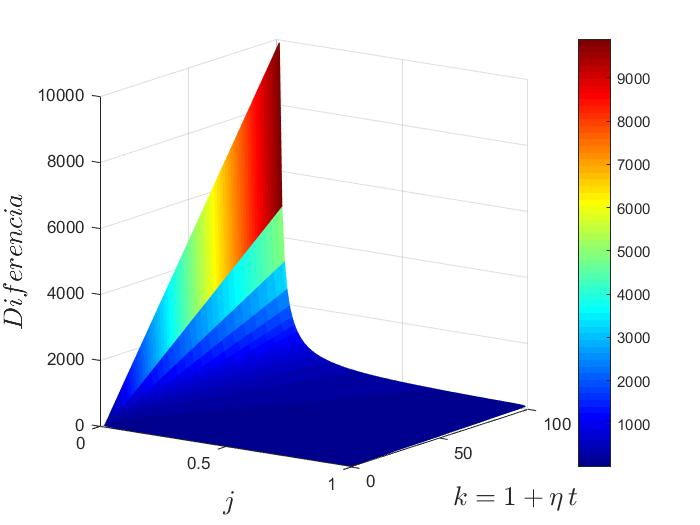
\includegraphics[width=0.495\textwidth]{5_Capitulo5/Graficos/Fig1.jpg}
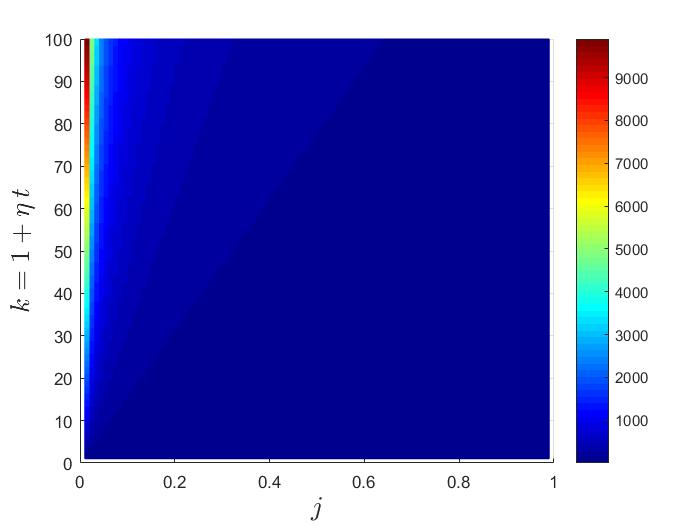
\includegraphics[width=0.495\textwidth]{5_Capitulo5/Graficos/Fig2.jpg}
%\vspace{-0.8cm} 
\caption{Gráfico de $d(k,j)$ para $(k,j) \in (0,100) \times  (0,1)$ .}
%\vspace{-0.8cm}
\label{fig_diferencia}
\end{center}
\end{figure}
% \begin{center}
% 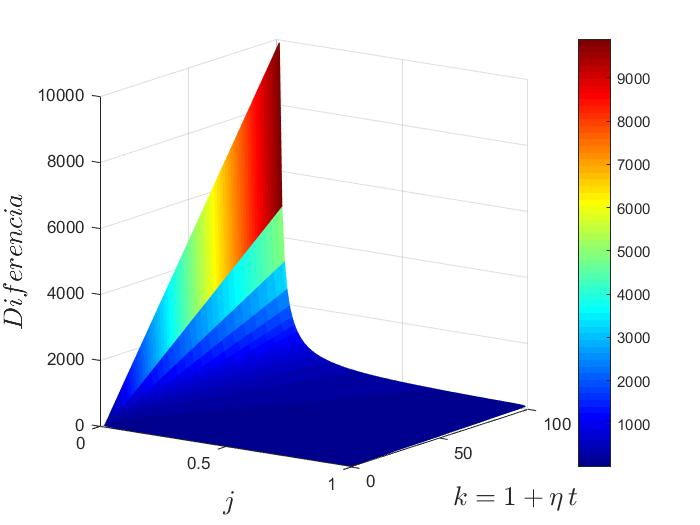
\includegraphics[scale=.4]{5_Capitulo5/Graficos/Fig1.jpg}
% 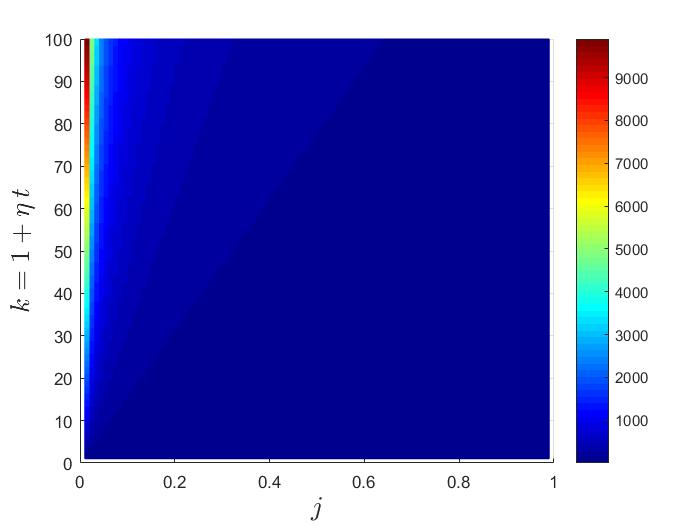
\includegraphics[scale=.4]{5_Capitulo5/Graficos/Fig2.jpg}
% \end{center}

En (\ref{fig_diferencia}) se puede observar que la función $d(k,j)$ es estrictamente positiva y que aumenta considerablemente para valores pequeños de $j$ y grandes de $k$.
Al verificar numéricamente que esta desigualdad es cierta, se procede al análisis de la segunda subcondición (\ref{sub_condi_pare_cuasi2}) para confirmar que  cumple la condición de Pareto (\ref{basic_condi_pareto_2}).

\subsection{Segunda subcondición}
En esta subsección, se llevará a cabo un análisis minucioso de la subcondición (\ref{sub_condi_pare_cuasi2}), ya que si se verifica, esto implica que se cumplen tanto (\ref{basic_condi_pareto}) como (\ref{basic_condi_pareto_2}).

Dado que, de acuerdo a (\ref{q_de_t_expo_integral}),
$$\exp\left(\ds \int_0^{T}q(t)dt\right)=(1+\eta T)^j+1,$$
como parte de la condición establecida, entonces,

$$\dfrac{1}{(1+\eta T)^j} >  \dfrac{1}{\exp\left(\ds \int_0^{T}I(t)dt\right)}=\dfrac{1}{(1+\eta T)^j+1} \Rightarrow
\dfrac{1}{(1+\eta T)^j} > \dfrac{1}{(1+\eta T)^j+1}.$$
Esta desigualdad se verifica puesto que $\eta>0$, $T>0$ y $j \in (0,1)$. 
% se cumple la desigualdad
% $$(1+\eta T)^j<(1+\eta T)^j+1.$$
Una vez constatada esta segunda subcondición, se puede afirmar con certeza que se cumplen (\ref{basic_condi_pareto}) y (\ref{basic_condi_pareto_2}).


\section{Revisión de la concavidad}
En esta sección, se llevará a cabo un análisis para determinar si el descuento cuasi-hiperbólico (\ref{c_hiper}) cumple con la condición para la concavidad del plan de consumo, tal como se establece en (\ref{prop 7}).

Las condiciones establecidas en la proposición (\ref{prop 7}) son que $\varepsilon(t) > -1$ y que $\mu(t)$ sea creciente, o de manera equivalente, que $\mu'(t) > 0$.

Dado que la primera condición ya ha sido demostrada en la sección (\ref{section_sesgo_presente}), se procede a analizar la segunda condición.
$$\dfrac{d}{dt}\left(\mu(t)\right)>0,$$
como se ve en (\ref{eq 86}) $\mu(t)$ es igual $\dfrac{\varepsilon'(t)}{1+\varepsilon'(t)}$ por lo cual se puede reescribir la desigualdad anterior como
$$\dfrac{d}{dt}\left(\dfrac{\varepsilon'(t)}{1+\varepsilon'(t)}\right)>0.$$
Dado que $\dfrac{\varepsilon'(t)}{1+\varepsilon'(t)}=\rho - \dfrac{j \eta}{(1+\eta t)}$, tal como se muestra en (\ref{deriv_var_mu_t}), entonces 
$$\dfrac{d}{dt}\left(\rho - \dfrac{j \eta}{(1+\eta t)}\right)=\dfrac{j\eta^2}{(1+\eta t)^2}>0.$$
Se considera que $t\geq 0$, $\eta>0$ y $j\in (0,1)$, se verifica que $j\eta^2>0$ y $(1+\eta t)^{2}\geq 1$. Por lo tanto, la segunda condición se encuentra satisfecha. Dadas ambas condiciones, se puede confirmar que el descuento cuasi-hiperbólico cumple la concavidad del plan de consumo.